\chapter{Código Limpo}\label{cap:cap3}

\begin{flushright}
	\textit{
		Um ladrão rouba um tesouro, mas não furta a inteligência. \\
		Uma crise destrói um herança, mas não uma profissão. \\ Não importa se você não tem dinheiro, você é uma pessoa rica, \\ pois possui o maior de todos os capitais: a sua inteligência. \\ Invista nela. \textbf{Estude}!.
	} \\
	
	\textbf{Augusto Cury}
\end{flushright}

\begin{figure}[H]
	\centering
	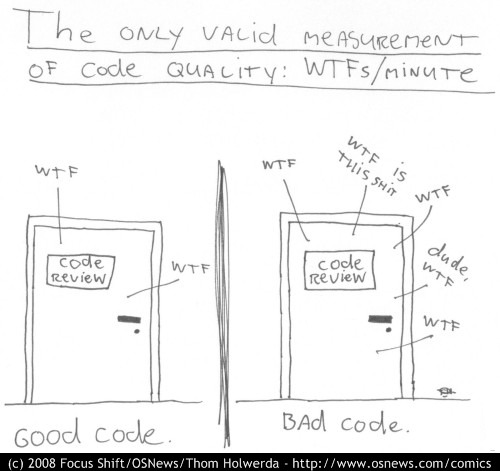
\includegraphics[scale=3.5]{imagens/687474703a2f2f7777772e6f736e6577732e636f6d2f696d616765732f636f6d6963732f7774666d2e6a7067.jpg}
\end{figure}

A imagem acima ilustra o livro ``Código Limpo'' de Robert Cecil Martin também conhecido com Uncle Bob. O livro é um guia para se produzir código \textbf{legível}, \textbf{reutilizável} e \textbf{refatorável}. Assim, baseando-se nesses conceitos, a ideia é demostrar o uso de alguns deles com a linguagem JavaScript.

Assim, citando um trecho do \href{https://github.com/felipe-augusto/clean-code-javascript}{Conceitos de Código Limpo adaptados em JavaScript} ``aprender isto não irá lhe transformar imediatamente em um desenvolvedor(a) de software melhor, trabalhar com eles por muitos anos não quer dizer que você não cometerá erros. Toda porção de código começa com um rascunho, como argila molhada sendo moldada em sua forma final. Finalmente, talhamos as imperfeições quando revisamos com nossos colegas. Não se sinta culpado pelos primeiros rascunhos que ainda precisam de melhorias. Ao invés, desconte em seu código''.

\section{O que é código limpo (Clean Code)}

Uma das atividades que as pessoas que desenvolvem softwares realizam além da codificação é a manutenções em sistemas. Para isso, é preciso fazer a leitura e o entendimento de inúmeros códigos fontes de programas desenvolvidos por outras pessoas. Essa atividade pode ser muito mais fácil de se executar caso o desenvolvimento seja feito com base em boas práticas de programação.

\textbf{Clean Code}, que significa código limpo, é uma técnica que cria um conjunto de práticas e orientações sobre como desenvolver códigos que sejam facilmente entendidos, escritos e mantidos pelas pessoas desenvolvedoras. O objetivo é garantir o desenvolvimento de aplicações com códigos de qualidade que possam ser facilmente reutilizados.

\section{Variáveis de Ambiente}

Se existe uma coisa que vários projetos de desenvolvimento tem em comum são dados sensíveis, como dados de acesso a banco de dados, chaves de API's, \textit{Secret Keys} entre outras dados de configuração necessárias. Como são dados críticos, eles não podem ter acesso público e, de forma alguma, podem estar em um repositório de dados aberto. 

Outro ponto são os ambientes de desenvolvimento. Quando o projeto está sendo executado e acessado por usuários dizemos que eles está em um \textbf{Ambiente de Produção - \textit{Production}}. Já, quando ele é executado pelos desenvolvedores dizemos que ele está em um \textbf{Ambiente de Desenvolvimento - Development}. Ambos possuem características semelhantes, mas executam de forma diferente. Assim, o banco de dados, por exemplo, que roda em \textbf{produção} tem acesso diferente ao banco que roda em \textbf{desenvolvimento}, logo, possui acesso (usuário e senha) diferente. Logo, nosso projeto, deve possuir essas características, e para isso vamos usar as \textbf{Variáveis de Ambiente}. 

\subsection{Dotenv}

O \textbf{Dotenv} é a ferramenta utilizada para separar as variáveis ambientes de um projeto. O nome dela sugere o arquivo em que as informações ficarão, \textbf{dot} que é ponto em inglês acrescido de \textbf{env}, então temos o arquivo \textbf{.env} que é composto de chaves e valores. Assim, para começar a usar, vamos instalar as dependências necessárias.

\begin{minted}[frame=single,framesep=10pt,breaklines,linenos,tabsize=2,autogobble]{javascript}
yarn add dotenv-safe
\end{minted}

Após a instalação, vamos criar um arquivo na raiz do projeto chamada \textbf{.env.exemplo}. Esse arquivo conterá as variáveis que vamos usar em nosso projeto. Todas elas devem, por padrão, serem em \textbf{maiúsculo} seguido do sinal de igual. 

\begin{minted}[frame=single,framesep=10pt,breaklines,linenos,tabsize=2,autogobble]{javascript}
# Váriáveis para o banco de dados
USUARIO=teste
SENHA=teste
\end{minted}

Já, para acessar-mos os dados das variáveis, em nosso arquivo principal, no topo, vamos adicionar o seguinte código que incorporará o Dotenv em nosso código.

\begin{minted}[frame=single,framesep=10pt,breaklines,linenos,tabsize=2,autogobble]{javascript}
require("dotenv-safe").config();
\end{minted} 

Com o arquivo \textbf{.env} configurado é necessário executar o Dotenv que irá chama-lo para ler as variáveis e adiciona-las ao processo que o executou, sabendo que para acessar as informações usem:

\begin{minted}[frame=single,framesep=10pt,breaklines,linenos,tabsize=2,autogobble]{javascript}
process.env.[NOME_DA_CHAVE]
process.env.SENHA
process.env.USUARIO
\end{minted}

Algumas observações para a criação das variáveis: 

\begin{itemize}[leftmargin=1.7cm]
	\setlength\itemsep{0em}
	\item As chaves são em caixa alta, por padrão e não exigência;
	\item As chaves não podem ter espaço;
	\item Os valores podem ser quaisquer tipo, que será retornado sempre uma string;
	\item Pode haver espaçamentos, porém é feito um trim na string;
	\item Pode existir chave sem valor, que retorna uma string vazia;
\end{itemize}

\subsection{Boas práticas e cuidados}

Por se tratar de informações sensíveis é importante que esses dados fiquem em seu ambiente de desenvolvimento, então se pretende compartilhar seu código, lembre-se de remover esse arquivo. Caso utilize o github basta adicionar ao .gitignore o arquivo .env para ele fazer esse trabalho para você.

Uma boa prática também é criar um arquivo de exemplo com as chaves que seu projeto está utilizando, sem os valores sensíveis, assim quem clonar o repositório ou ter acesso ao seu fonte não ficará perdido.Crie um \textbf{.env.example} e deixo apenas as variáveis de ambiente sem seus respectivos valores.

\section{Aplicação de código limpo em variáveis, funções e classes}
